\documentclass[12pt,a4paper,titlepage,oneside]{report}

%%{{{ packages
%% font encoding.
\usepackage[utf8]{inputenc}
\usepackage[T1]{fontenc}
\usepackage{lmodern}
\usepackage{couriers}
%% Customize chapters.
\usepackage{titlesec}
%% bibliography.
\usepackage[backend=bibtex,style=ieee]{biblatex}
%% \includegraphics{name}
\usepackage{graphicx}
%% \url{something}
\usepackage{url}
%% \multirow{package}{width}{text}
\usepackage{multirow}
%% \cellcolor
\usepackage[table]{xcolor}
%% \caption{title}
\usepackage{caption}
\usepackage{subcaption}
%% \forloop
\usepackage{forloop}
%% fix underfull on footnote with URL.
\usepackage{ragged2e}
%% source code listing
\usepackage{listings}
%% \printindex
\usepackage{makeidx}
%% table of content
\usepackage{tocloft}
%% text emphasis, including strikeout.
\usepackage[normalem]{ulem}
%% mathematics
\usepackage{mathtools}
%% arithmetic
\usepackage{calc}
%% algorithm
\usepackage{algorithm}
\usepackage{algpseudocode}
%% multiple columns
\usepackage{multicol}
%% Change the margin
\usepackage[a4paper]{geometry}
\geometry{
	a4paper,
	top=3cm,
	right=3cm,
	bottom=3cm,
	left=4cm
}
%%
\usepackage{parskip}
%% Package for reading CSV to database.
\usepackage{datatool}
%% Package for scatter and line plot.
\usepackage{dataplot}
%% Long table
\usepackage{longtable}
%% Tikz
\usepackage{pgfplots}

%% Add box to figure.
%%
\usepackage{float}

\floatstyle{boxed}
\restylefloat{figure}

%% MnSymbol
\usepackage{MnSymbol}
%%}}}

%%{{{ hyphenation: sorted in ascending.
%%
\hyphenation{
	Ja-nu-a-ri
	SIGKDD
	Wiki-pedia
	a-kan
	ang-ka
	ba-gai-ma-na
	bayes-ian
	ber-kas
	ber-ma-sa-lah
	ber-mak-na
	bi-a-ya
	da-lam
	data-set
	de-ngan
	di-ha-sil-kan
	di-sing-kat
	di-tam-bah-kan
	dis-krit
	fung-si
	ga-bung-an
	ke-las
	ke-mung-ki-nan
	ke-tak-se-imbang-an
	lan-guage
	ma-yo-ri-tas
	me-laku-kan
	me-me-rik-sa
	me-mi-lih
	me-ne-rap-kan
	me-ning-kat-kan
	me-nye-dia-kan
	me-nye-im-bang-kan
	me-sin
	me-thod
	mem-vi-sua-li-sa-si
	meng-gu-na-kan
	meng-hu-bung-kan
	meng-i-kut-kan
	meng-i-kuti
	meng-im-ple-men-ta-si-kan
	meng-in-di-ka-si-kan
	mi-sal-nya
	mung-kin
	o-ver-sam-pling
	pa-ra-lel
	pe-mi-sah
	pe-nan-da
	pe-ne-li-ti-an
	pe-nu-li-san
	pe-nyun-ting
	pem-ban-ding
	pen-de-kat-an
	peng-kla-si-fi-ka-si
	per-for-man-si-nya
	po-ten-si-al
	pro-ba-bi-li-tas
	pro-ses
	sam-pel
	se-im-bang
	se-jum-lah
	sun-ting-an
	ting-kat
	un-der-sam-pling
	wa-lau-pun
}
%%}}}

%%{{{ override default latex setting.
%%

%% Space between paragraphs.
\setlength{\parskip}{1.5em}

%% Add dot to TOC.
\renewcommand{\cftsecleader}{\cftdotfill{\cftdotsep}}
\renewcommand{\contentsname}{}

\lstset{
	basicstyle=\scriptsize\ttfamily
,	breaklines=true
,	stringstyle=\scriptsize\ttfamily
,	numbers=left
,	numberstyle=\tiny\ttfamily
,	numbersep=5pt
,	tabsize=4
,	frame=single
}

\makeatletter
\def\lst@lettertrue{\let\lst@ifletter\iffalse}
\makeatother

%% Format chapter and section.
%%
%%% Set chapter name to Bab.
\titleformat{\chapter}[hang]
{\bfseries\large\centering}
{Bab \thechapter}
{1em}
{}

\titleformat{\section}[hang]
{\bfseries\large}
{\thesection}
{1em}{}

%% Set spacing for sections.
\titlespacing{\chapter}{0ex}{0ex}{1.5em}
\titlespacing{\section}{0ex}{0ex}{0em}

%% Alter latex default title on table.
\captionsetup[table]{name=Tabel}
\captionsetup[figure]{name=Gambar}

\renewcommand{\arraystretch}{1.5}
\setlength{\tabcolsep}{3pt}

%% Change bibliography title.
\defbibheading{bibliography}{\centerline{
	\textbf{DAFTAR REFERENSI}}
}

%%% uncomment this to show overrule in black box
\overfullrule=2cm

%% Algorithmicx
\makeatletter
\renewcommand{\ALG@beginalgorithmic}{\footnotesize}
\makeatother

%% multicolumn setting
\setlength{\columnsep}{1cm}

%% pgfplots setting.
\pgfplotsset{
	/pgf/number format/read comma as period,
	/pgf/text mark as node=false,
	table/col sep=semicolon,
	xmax=1,
	xmin=0,
	ymax=1,
	ymin=0,
	xtick distance=0.2,
	ytick distance=0.2,
	grid=major,
	cycle list name=linestyles,
}
%%}}}

%%{{{ variables
%%
\newcommand{\mytitle}{Deteksi Vandalisme pada Wikipedia Bahasa Inggris menggunakan klasifikasi Cascaded Random Forest}
\newcommand{\myname}{Muhamad Sulhan}
\newcommand{\mysid}{23513014}
\newcommand{\myadvisorname}{Dwi Hendratmo Widyantoro}
\newcommand{\myadvisorid}{196812071994021001}
\newcommand{\mydept}{Program Studi Magister Informatika}
\newcommand{\itb}{Institut Teknologi Bandung}

%%% My images directory
\graphicspath{{../images/}}
\newcommand{\myitbcover}{ITB-logo-hitam}

%%% My bibligraphy file
\addbibresource{bibliography.bib}
%%}}}

%%{{{ document's meta-data
%%
\author{\myname}
\title{\mytitle}
%%}}}

%%{{{ document's macros
%%
%%% two column signature.
\def\myadvisorsig#1{%
	\vbox{\hsize=6cm
		\textbf{#1}\\
		\addvspace{2cm}%
		\hbox to \hsize{%
			\strut\hfil%
			\myadvisorname%
			\hfil%
		}
		\hrule\kern1ex
		\hbox to \hsize{%
			\strut\hfil%
			NIP\hspace{1ex}\myadvisorid%
			\hfil%
		}
	}
}

%%% one column signature.
\def\mysignature#1#2#3{%
	\vbox{
		\textbf{#1}\\
		\addvspace{2cm}%
		\hbox to \hsize{%
			\strut\hfil%
			{#2}%
			\hfil%
		}
		\makebox[6cm][c]{
			\hrulefill
		}
		\hbox to \hsize{%
			\strut\hfil%
			NIP\hspace{1ex}{#3}%
			\hfil%
		}
	}
}

%%% source code listing
\lstdefinelanguage{go}
{
	morekeywords={package,import,const,func,for,type,var,struct}
,	sensitive=true
,	morecomment=[l]{//}
,	morecomment=[s]{/*}{*/}
}
\lstdefinestyle{go}{%
	language=go
,	keywordstyle=\color{black}\bfseries
,	commentstyle=\color{gray}
,	breakatwhitespace=true
,	lineskip={-2.5pt}
}
\newcommand{\includecodego}[2][c]{
	\lstinputlisting[caption=#2,escapechar=,style=go]
		{/home/ms/go/work/src/github.com/shuLhan/#2}
}

%%% data listing
\lstdefinestyle{data}{%
	breakatwhitespace=false
,	breakautoindent=false
,	literate={\,}{}{0\discretionary{,}{}{,}},
}
\newcommand{\includedata}[2][c]{
	\lstinputlisting[caption=#2,style=data,linerange={1-10}]
		{/home/ms/go/work/src/github.com/shuLhan/#2}
}
%%}}}

%%
%% Create cover with parameters
%% 1: report number
%% 2: report weeks, in string
%% 3: report date, string
%%
\newcommand{\reportcover}[3]{
	\thispagestyle{empty}
	\begin{center}\textbf{%
		\mytitle
		\vfill
		Laporan Progres Tesis, Catatan, dan Pekerjaan Selanjutnya
		\linebreak
		Laporan ke-#1
		\linebreak
		Minggu #2
		\linebreak
		\linebreak
		#3
		\vfill
		Oleh \\
		\myname \\
		\mysid \\
		\vfill
		\uppercase{%
			Program Studi Magister Informatika \\
			Sekolah Teknik Elektro dan Informatika \\
			Institut Teknologi Bandung \\
			2015
		}
	}
	\end{center}
	\newpage
}

%%
%% Macro for advisor's signature
%%
\newcommand{\advisorsignature}{
	\vfill
	\begin{center}
		Diketahui oleh,
		\linebreak
		\linebreak
		\hbox to \hsize{%
			\myadvisorsig{Pembimbing,\quad}\hfil
		}
	\end{center}
}

%%
%% Macro for create schedule using parameter
%% 1: number of weeks has passed on task 1
%% 2: number of weeks has passed on task 2
%% 3: number of weeks has passed on task 3
%% 4: number of weeks has passed on task 4
%% 5: should we begin in newpage?
%%

% function to fill cell with color
\newcommand{\tand}{&}
\newcounter{cnt}
\newcommand{\fillcell}[1]{%
	\forloop{cnt}{0}{\value{cnt}<#1}{%
		{\cellcolor[gray]{0.7}} \tand
	}%
}
% function to create empty cell
\newcommand{\emptycell}[2]{%
	\forloop{cnt}{0}{\value{cnt}<#1}{%
		\tand
	}%
	\ifthenelse{#2 = 1}{\\}{\tand}%
}
% function to fill week in progress.
\newcommand{\progresscell}[1]{%
	\forloop{cnt}{0}{\value{cnt}<#1}{%
		{\cellcolor{red!80}} \tand
	}%
}

\newcommand{\schedule}[4]{
	\section{Penjadwalan}\label{sec:penjadwalan}

Tabel di bawah menampilkan jadwal yang direncanakan dalam pengembangan tesis dari bulan ke I, September 2015, sampai dengan bulan ke VI, Januari 2016.

Warna merah menandakan minggu yang telah lewat sampai minggu dari laporan progres ini, untuk warna abu-abu menandakan waktu pelaksanaan yang akan datang.

\newcounter{planone}
\newcounter{plantwo}
\newcounter{planthree}
\newcounter{planfour}

\newcounter{progressone}
\newcounter{progresstwo}
\newcounter{progressthree}
\newcounter{progressfour}

\setcounter{progressone}{#1}
\setcounter{progresstwo}{#2}
\setcounter{progressthree}{#3}
\setcounter{progressfour}{#4}

\setcounter{planone}{4 - \theprogressone}
\setcounter{plantwo}{17 - \theprogresstwo}
\setcounter{planthree}{14 - \theprogressthree}
\setcounter{planfour}{2 - \theprogressfour}

\begin{table}[h!]
	\centering
	{\footnotesize
	\begin{tabular}{|c|p{0.2\textwidth}
	|c|c|c|c
	|c|c|c|c
	|c|c|c|c
	|c|c|c|c
	|c|c|c|c
	|c|c|c|c|}
		\hline
		\multirow{2}{*}{No.}
			& \multirow{2}{*}{Kegiatan}
			& \multicolumn{4}{c|}{Bulan I}
			& \multicolumn{4}{c|}{Bulan II}
			& \multicolumn{4}{c|}{Bulan III}
			& \multicolumn{4}{c|}{Bulan IV}
			& \multicolumn{4}{c|}{Bulan V}
			& \multicolumn{4}{c|}{Bulan VI}\\
		\cline{3-26}
		& &
			1 & 2 & 3 & 4 &
			1 & 2 & 3 & 4 &
			1 & 2 & 3 & 4 &
			1 & 2 & 3 & 4 &
			1 & 2 & 3 & 4 &
			1 & 2 & 3 & 4\\
		\hline
		1 & Persiapan\ \  Data dan\ \ Lingkungan Penelitian &
			\progresscell{\theprogressone}
			\fillcell{\theplanone}
			\emptycell{19}{1}
		\hline
		2 & Implementasi dan Pengujian &
			\emptycell{2}{0}
			\progresscell{\theprogresstwo}
			\fillcell{\theplantwo}
			\emptycell{3}{1}
		\hline
		4 & Analisis &
			\emptycell{7}{0}
			\progresscell{\theprogressthree}
			\fillcell{\theplanthree}
			\emptycell{1}{1}
		\hline
		5 & Evaluasi &
			\emptycell{20}{0}
			\progresscell{\theprogressfour}
			\fillcell{\theplanfour}
			\emptycell{0}{1}
		\hline
	\end{tabular}
	}
	\caption{Jadwal penelitian tesis}
\end{table}
}




%%
%% DOCUMENT
%%
\begin{document}
\reportcover{3}{5 dan 6}{16 Oktober 2015}
\tableofcontents

%%{{{ Progress summary.
%%
\section{Laporan Progres}

Bagian ini mencatat rangkuman dari progres pekerjaan yang telah dilakukan setiap minggu.
Rincian dari progres berada pada bagian \ref{sec:catatan}.

\subsection{Minggu I}

\begin{itemize}
	\item \textbf{Data korpus untuk PAN-WVC-11 telah diunduh.}
Ukuran berkas terkompres yaitu 371 MB, dan tidak terkompres sebesar 1,1 GB.
Jumlah suntingan yaitu 9985, dengan 8734 diantaranya adalah suntingan regular dan 1251 (sekitar 12\%) adalah vandalisme.

	\item \textbf{Perbaikan proposal tesis.}
\end{itemize}

\subsection{Minggu II}

\begin{itemize}
	\item \textbf{Data korpus untuk PAN-WVC-10 telah diunduh.}
Ukuran berkas terkompres yaitu 439 MB, dan tidak terkompres sebesar 1,3 GB.
Jumlah dataset yaitu 32439 revisi, dengan 30045 diantaranya adalah suntingan regular dan 2394 (sekitar 7\%) diantaranya adalah vandalisme.

	\item \textbf{Pemasangan \textit{Database Management System} (DBMS).}
DBMS yang digunakan adalah MariaDB, yang merupakan \textit{fork} dari MySQL.
DBMS nantinya digunakan untuk menyimpan data ekspor dari hasil \textit{dump} riwayat penyuntingan Wikipedia.
Wikimedia (perangkat lunak wiki yang digunakan oleh Wikipedia), menggunakan MySQL sebagai DBMS, itulah kenapa MariaDB dipilih dalam pengembangan tesis ini.

	\item \textbf{Data \textit{dump} dari riwayat wikipedia telah diunduh.} \footnote{\RaggedRight\url{http://dumps.wikimedia.org/enwiki/20150805/enwiki-20150805-stub-meta-history1.xml.gz}}
Berkas hanya satu dari 27 berkas \textit{dump} yang memiliki total 43,5 GB.
Ukuran data terkompres yaitu 503 MB dan tidak terkompres 3,3 GB.
Format data berupa xml.
\end{itemize}

\subsection{Minggu III}

\begin{itemize}
	\item Menambah lampiran yang menampilkan contoh data dari PAN-WVC-10 dan PAN-WVC-11.
	\item Eksplorasi fitur-fitur yang digunakan untuk klasifikasi yang telah digunakan oleh makalah-makalah sebelumnya dan memperkirakan fitur yang akan digunakan pada tesis ini.
Mengembangkan sebuah fitur membutuhkan waktu, sebagai tahap awal hanya akan menggunakan 20 fitur yaitu 4 fitur metadata, 11 fitur teks, dan 5 fitur bahasa yang diambil dari hasil analisis makalah Mola-Velasco \cite{mola2012wikipedia}. Pada saat implementasi sudah berjalan dengan benar, baru nanti secara iteratif ditambahkan fitur-fitur dari makalah lainnya satu persatu.
\end{itemize}

\subsection{Minggu IV}

Telah membaca makalah tentang SMOTE \cite{chawla2002smote} dan LN-SMOTE \cite{maciejewski2011local} dan membuat rangkuman tentang perbedaan dari kedua metode tersebut berdasarkan kekurangan dan solusi yang diajukan dalam makalah.

\subsection{Minggu V, VI}

Implementasi algoritma SMOTE pada bahasa pemrograman Go. Sumber kode dapat dilihat pada lampiran.

%%
%%}}}

%%{{{ Notes
\newpage
\section{Catatan} \label{sec:catatan}

Bagian ini berisi pengetahuan yang didapat pada setiap minggu selama mengerjakan tesis.

\subsection{Minggu I dan II}
Korpus PAN-WVC-10 terbagi menjadi dua yaitu dataset suntingan dan dataset anotasi yang berisi hasil klasifikasi.
Kedua dataset memiliki format yang sama yaitu menggunakan \textit{Coma Separated Value} (CSV).
Dataset suntingan memiliki atribut sebagai berikut,
\begin{itemize}
	\item \textbf{editid}, format angka, berisi identifikasi (ID) unik dari setiap suntingan.
	\item \textbf{editor}, format string, berisi nama penyunting.
	\item \textbf{oldrevisionid}, format angka, berisi ID untuk suntingan lama.
	\item \textbf{newrevisionid}, format angka, berisi ID untuk suntingan baru.
	\item \textbf{diffurl}, format string, berisi URL yang mengacu pada perbedaan suntingan baru dengan lama.
	\item \textbf{edittime}, format string, berisi tanggal dan pukul sesuai dengan ISO 8601.
	\item \textbf{editcomment}, format string, berisi komentar yang ditambahkan oleh penyunting saat menyimpan hasil suntingan.
	\item \textbf{articleid}, format angka, berisi ID unik dari artikel.
	\item \textbf{articletitle}, format string, berisi judul dari artikel yang disunting.
\end{itemize}

Dataset anotasi memiliki atribut sebagai berikut,
\begin{itemize}
	\item \textbf{editid}, format angka, mengacu pada ID yang sama pada dataset suntingan.
	\item \textbf{class}, format string, berisi tipe suntingan yang bernilai "regular" yang menyatakan bahwa suntingan tersebut bukan vandalisme, dan "vandalism" yang menyatakan bahwa suntingan tersebut adalah vandalisme.
	\item \textbf{annotators}, format angka, berisi jumlah orang yang menandai (penanda) bahwa suntingan dengan ID tersebut termasuk ke dalam kelas "regular" atau "vandalism".
	\item \textbf{totalannotators}, format angka, berisi jumlah total penanda yang memeriksa suntingan.
\end{itemize}

Korpus PAN-WVC-11 hanya memiliki satu dataset untuk Bahasa Inggris yaitu dataset suntingan, dengan atribut yang menggabungkan dataset suntingan dan dataset anotasi pada PAN-WVC-10.

Rencananya, korpus PAN-WVC-10 dijadikan sebagai dataset untuk \textit{resampling} dan pelatihan klasifikasi karena kuantitasnya lebih banyak daripada PAN-WVC-11.
Korpus PAN-WVC-11 dijadikan sebagai dataset untuk pengujian model.

Contoh data untuk korpus PAN-WVC-10 dan PAN-WVC-11 dapat dilihat pada lampiran \ref{appendix:korpus}.


\subsection{Minggu III}
\subsubsection{Eksplorasi Fitur Vandalisme pada Wikipedia}

Beberapa makalah sebelumnya mengelompokan fitur-fitur ke dalam kelompok \textit{metadata}, teks, dan bahasa.
Sebagai tahap awal digunakan empat 4 metadata, 11 fitur teks, dan 5 fitur bahasa yang diambil dari hasil analisis makalah Mola-Velasco \cite{mola2012wikipedia}.

\paragraph{Fitur Kelompok Metadata}

Kelompok metadata mengacu pada properti dari sebuah revisi yang secara langsung dapat diambil, seperti identitas penyunting, atau waktu suntingan.

Berikut daftar fitur-fitur yang dapat digunakan pada klasifikasi vandalisme berbasiskan metadata,

\begin{itemize}

\item \textbf{Anonim}.
Melihat apakah penyunting memiliki akun atau anonim (hanya tercatat alamat \textit{IP}-nya).
Vandal lebih condong berlaku anonim karena jika menggunakan akun asli akan membuat akun mereka mudah diblokir.

\item \textbf{Panjang komentar}.
Melihat dari jumlah karakter yang digunakan di kolom "rangkuman suntingan" saat menyimpan hasil suntingan.
Komentar yang panjang mungkin mengindikasikan suntingan biasa dan yang pendek atau kosong mungkin menyarankan suatu vandalisme.
Namun, fitur ini sedikit lemah karena banyak suntingan biasa meninggalkan komentar yang kosong.

\item \textbf{Peningkatan ukuran}.
Peningkatan absolut dari ukuran konten artikel, dihitung dengan
\[
|ukuran\ suntingan\ baru| - |ukuran\ suntingan\ lama|
\]
Misalnya, berkurangnya ukuran dalam jumlah besar bisa mengindikasikan pengosongan artikel.

\item \textbf{Rasio ukuran}.
Ukuran revisi baru relatif terhadap revisi lama, yaitu
\[
\frac{1 + |baru|}{1 + |lama|}
\]

\end{itemize}

\paragraph{Fitur Kelompok Teks}

Berikut daftar fitur-fitur yang dapat digunakan pada klasifikasi vandalisme berbasiskan teks,

\begin{itemize}

\item \textbf{Rasio huruf besar dan kecil}.
Pelaku vandal biasanya tidak mengikuti aturan huruf kapital, menulis semuanya dengan huruf kecil atau huruf besar.
Rasio ini dihitung dengan menggunakan rumus
\[
\frac{1 + |perubahan\ baru|}{1 + |perubahan\ lama|}
\]

\item \textbf{Rasio huruf besar terhadap semua huruf}
Rasio ini dihitung dengan menggunakan rumus
\[
\frac{1 + |huruf\ besar|}{1 + |huruf\ besar| + |huruf\ kecil|}
\]

\item \textbf{Rasio angka}.
Rasio semua karakter terhadap angka, yaitu
\[
\frac{1 + |angka|}{1 + |semua|}
\]
Fitur ini membantu menemukan suntingan kecil yang hanya mengubah angka.
Contoh kasusnya perubahan sebuah tanggal atau perhitungan untuk menyebabkan kesalahan informasi.

\item \textbf{Rasio non-alfanumerik}.
Rasio semua karakter terhadap karakter selain huruf dan angka, yaitu
\[
\frac{1 + |non\ alfanumerik|}{1 + |semua\ karakter|}
\]
Kelebihan penggunaan karakter selain angka-huruf bisa mengindikasikan penggunaan \textit{emoticon}, tanda baca, atau kata tak bermakna.

\item \textbf{Diversitas karakter}.
Menghitung karakter berbeda dibandingkan dengan panjang teks yang dimasukan, yaitu
\[
length \frac{1}{karakter\ berbeda}
\]
Fitur ini membantu menemukan penggunaan karakter secara acak dan kata tak bermakna.

\item \textbf{Distribusi karakter}.
Menggunakan Divergensi Kullback-Leibler dari distribusi karakter yang dimasukan terhadap ekspektasi.
Fitur ini berguna untuk mendeteksi kata tak bermakna.

\item \textbf{Kompresabilitas}.
Melihat tingkat kompres dari teks menggunakan algoritma LZW.
Fitur ini berguna untuk mendeteksi kata tak bermakna, pengulangan kata atau karakter, dll.
Vandalisme biasanya memiliki ukuran kompresi yang rendah.

\item \textbf{Token umum}.
Token yang biasanya jarang digunakan oleh vandal adalah sintaks wiki, seperti \textit{\_\_TOC\_\_}.

\item \textbf{Frekuensi rerata kata}.
Frekuensi relatif rerata dari kata yang dimasukan pada revisi baru.
Pada artikel yang panjang, semakin banyak kata yang dimasukan yang tidak ada pada artikel mengindikasikan bahwa suntingan tersebut bisa tak bermakna atau tidak berhubungan dengan isinya.

\item \textbf{Kata terpanjang}.
Panjang dari kata yang dimasukan.
Nilainya akan 0 jika tidak ada kata yang dimasukan.
Fitur ini berguna untuk mendeteksi suntingan tak-bermakna.

\item \textbf{Urutan karakter terpanjang}.
Urutan terpanjang dari karakter yang sama pada teks yang dimasukan sering digunakan pada vandalisme, contohnya \textit{aaarrrrggghhh! sooo huge}.

\end{itemize}

\paragraph{Fitur Kelompok Bahasa}

Fitur kelompok bahasa berdasarkan jumlah kata yang ditambahkan pada suntingan baru.
Dua fitur berikut dihitung relatif terhadap konten yang baru: frekuensi dan dampak.
Frekuensi adalah menghitung frekuensi dari kata tersebut dari total seluruh kata pada suntingan yang baru.
Dampak adalah menghitung persentase penambahan jumlah kata tersebut pada suntingan.
Berikut daftar fitur-fitur yang dapat digunakan pada klasifikasi vandalisme berbasiskan bahasa,

\begin{itemize}
\item \textbf{Vulgarisme}.
Menghitung kata-kata vulgar dan menghina, misalnya \textit{fuck}, \textit{suck}, \textit{stupid}.

\item \textbf{Subjek}.
Menghitung kata-kata subjek pertama atau kedua, termasuk pengejaan tidak baku, misalnya \textit{I}, \textit{you}, \textit{ya}.

\item \textbf{Bias}.
Menghitung penggunaan kata sehari-hari yang mengandung bias, misalnya \textit{coolest}, \textit{huge}.

\item \textbf{Seks}.
Menghitung penggunaan kata berhubungan dengan seks, misalnya \textit{sex}, \textit{penis}, \textit{nipple}.

\item \textbf{Kata buruk}.
Gabungan kategori untuk kata sehari-hari dan beberapa penulisan yang buruk (misalnya, \textit{wanna}, \textit{gotcha}).

\end{itemize}

\subsubsection{Eksplorasi Sumber Kode Referensi}

Penulis menemukan sumber kode yang digunakan oleh referensi utama
\footnote{
	\url{https://github.com/webis-de/wikipedia-vandalism-detection}
}.
Setelah mengunduh sumber kode dan mempersiapkan ketergantungan yang dibutuhkan untuk menjalankan aplikasi tersebut (seperti bahasa pemrograman dan semua ketergantungan pustaka yang dibutuhkan), penulis tidak dapat menjalankan sumber kode karena ada ketergantungan atau konfigurasi yang mungkin terlewat atau tidak tertulis sehingga tidak dapat menjalankan program.

Penulis masih mencoba memperbaiki kesalahan tersebut untuk tiga hari mendatang.
Seandainya masih tidak bisa, setidaknya ada gambaran bagaimana penerapan teknik \textit{resampling} dan penggunaan klasifikasi dilakukan.


\subsection{Minggu IV}
\subsubsection{Metode SMOTE}

Metode \textit{Synthetic Minority Over-sampling Technique} (SMOTE)
\parencite{chawla2002smote} menggunakan pendekatan \textit{over-sampling} yang mana
kelas minoritas ditambah dengan membuat sampel sintetis, bukan dengan
mengganti sampel dari kelas mayoritas menjadi kelas minoritas.
Sampel sintetis dibuat lewat aplikasi dengan beroperasi pada
ruang fitur.
Kelas minoritas ditambah dengan mengambil setiap sampel-sampel dari kelas
minoritas dan membuat sampel sintetis di antara segmen garis yang menghubungkan
setiap $k$ tetangga terdekat (\textit{k-nearest-neighbors}, KNN) dari kelas
minoritas.
Instan dari KNN dipilih secara acak, bergantung dari jumlah
\textit{over-sampling} yang dibutuhkan.

\begin{figure}[htbp]
\centering
\setlength\fboxsep{4pt}
\fbox{
	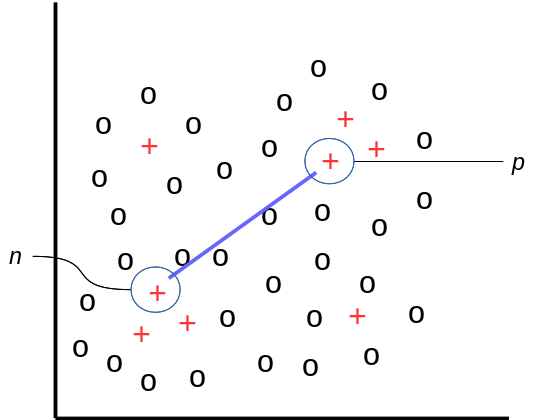
\includegraphics[keepaspectratio=true,scale=0.35]{SMOTE-example}
}
	\caption{
	Ilustrasi pembuatan sampel sintetis pada SMOTE.
	Misalkan $p$ adalah sampel minoritas dan $n$ adalah salah satu dari $k$
	tetangga terdekat dari $p$, maka
	sampel sintetis yang baru akan berada di garis antara $p$ dan $n$.
	}
	\label{fig:smote}
\end{figure}

Sampel sintetis dibuat dengan cara berikut, misalkan $p$ adalah salah satu
sampel minoritas pada dataset $D$,
\pagebreak
\begin{itemize}
	\item Cari $k$ sampel tetangga dari $p$ pada $D$
	\item Untuk setiap sampel tetangga $k$,
	\begin{itemize}
		\item Hitung selisih antara vektor fitur $p$ dengan tetangga $k_{i}$
		\item Kalikan selisih tersebut dengan angka ril acak antara 0 sampai 1,
		dan
		\item simpan hasilnya ke vektor fitur sintentis yang baru.
	\end{itemize}
\end{itemize}

Cara ini membuat sampel secara acak pada segmen garis antara dua fitur yang
terpilih, seperti yang terlihat pada gambar \ref{fig:smote}.
Pendekatan ini secara efektif mendorong wilayah pembelajaran dari kelas
minoritas menjadi lebih besar tanpa menyebabkan \textit{overfitting}.


\subsubsection{Metode LN-SMOTE}

Meskipun hasil SMOTE dibuktikan bagus dalam makalah Chawla dkk.
\cite{chawla2002smote}, metode ini masih memiliki beberapa kelemahan.
Pertama, cara menentukan sampel minoritas sebagai calon untuk
\textit{over-sampling} bisa bermasalah.
Pada SMOTE, semua sampel dari kelas minoritas digunakan.
Namun, bukan berarti semua sampel tersebut sama bergunanya bagi pembelajaran
klasifikasi.
Pada khususnya, sampel yang ada pada batas \textit{decision}, atau berada
dibatas kelas minoritas dengan kelas mayoritas, lebih sering salah
diklasifikasi dibandingkan dengan sampel yang berada jauh dari batas kelas,
oleh karena itu mereka lebih penting untuk klasifikasi.
Sampel yang jauh dari batas kelas, berada di tengah kelas minoritas mungkin
berkontribusi sedikit pada klasifikasi.
Salah satu metode untuk menangani permasalahan ini yaitu dengan hanya
mengambil sampel pada batas kelas minoritas yang dijadikan untuk
\textit{oversampling}, seperti yang diajukan oleh Han dkk.
\cite{han2005borderline} dengan menggunakan metode bernama \textit{Borderline
SMOTE}.

\begin{figure}[htbp]
	\centering
	\begin{subfigure}[b]{0.4\textwidth}
		\centering
		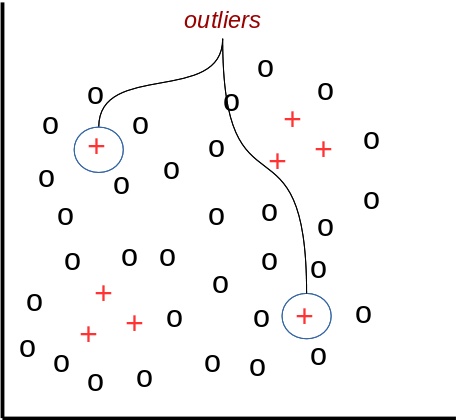
\includegraphics[width=\textwidth]{SMOTE-problem-outliers}
		\caption{}
		\label{fig:smote-outliers}
	\end{subfigure}
	\begin{subfigure}[b]{0.5\textwidth}
		\centering
		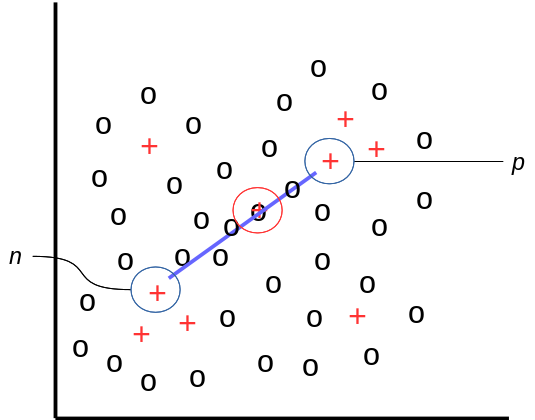
\includegraphics[width=\textwidth]{SMOTE-problem-overlapping}
		\caption{}
		\label{fig:smote-overlapping}
	\end{subfigure}
	\caption{
Kelemahan metode SMOTE:
(a) \textit{Outliers} pada kelas minoritas tidak diperhitungkan pada metode
SMOTE.
(b) Pembuatan sampel sintetis yang baru berada di wilayah kelas mayoritas
yang tumpang-tindih dengan sampel kelas mayoritas.
	}
	\label{fig:smote-problems}
\end{figure}

Kelemahan lain dari SMOTE yaitu permasalahan \textit{overgeneralization} yang
begitu saja menggeneralisasi wilayah dari kelas minoritas.
SMOTE tidak mempertimbangkan distribusi dari sampel pada kelas mayoritas, atau
adanya \textit{outliers}.

Untuk mengatasi permasalahan di atas, Maciejewski dkk. memperkenalkan ekstensi
dari metode SMOTE bernama \textit{Local-neighbourhood SMOTE} atau disingkat
LNSMOTE \cite{maciejewski2011local} yang menggunakan modifikasi dari
pendekatan \textit{Safe-Level SMOTE} \cite{bunkhumpornpat2009safe}.
Pada metode \textit{Safe-level SMOTE} keberadaan sampel mayoritas
diperhitungkan sebelum membuat sampel sintetis dengan menghitung sebuah
koefisien khusus yang disebut \textit{safe level}.
Untuk setiap sampel dari kelas minoritas, dihitung jumlah sampel kelas
minoritas di antara \textit{k-nearest-neighbors} (KNN).
Jika nilainya sama atau mendekati $ 0 $, sampel tersebut dianggap sebagai
\textit{noise}.
Jika nilainya mendekati $ k $, maka sampel tersebut bisa dikatakan berada
di wilayah aman dari kelas minoritas.
Gagasan utamanya adalah membuat sampel sintetis yang dekat dengan wilayah aman.

Lebih rincinya, misalkan $ p $ adalah sampel dari kelas minoritas yang akan
menjadi calon untuk \textit{over-sampling}, maka $ k $ sampel terdekat dengan
$ p $ yang termasuk pada kelas minoritas $ P $ ditentukan.
Seperti pada SMOTE, setidaknya satu dari tetangga tersebut dipilih, sebutlah
dengan $ n $.
Untuk kedua sampel, $ p $ dan $ n $, $ k $ sampel terdekatnya untuk keseluruhan
data pelatihan $ S $ dihitung \textit{safe level}-nya dengan notasi $ sl(p) $
dan $ sl(n) $.
Dari pengetahuan tersebut, koefisien rasio \textit{safe-level} ditentukan
dengan $ \textit{sl-ratio} = sl(p) / sl(n) $.
Langkah selanjutnya ditentukan berdasarkan 5 kasus berikut:
\begin{enumerate}
	\item \label{case:safe-1} Jika $ sl(p) = 0 $ dan $ sl(n) = 0 $, sampel
	$ p $ dan $ n $ dianggap sebagai \textit{noise outliers}, dan tidak ada
	sampel sintetis yang dibuat.
	\item Jika $ sl(p) > 0 $ dan $ sl(n) = 0 $, maka $ n $
	adalah \textit{noise}.
	Sampel sintetis akan dibuat jauh dari $ n $ dengan menduplikasi $ p $.
	\item Jika $ sl-ratio = 1 $, maka $ p $ dan $ n $ memiliki tetangga
	yang sama dan sampel sintetis yang baru akan dibuat diantara garis yang
	menghubungkan mereka dengan cara yang sama seperti pada SMOTE.
	\item Jika $ sl-ratio > 1 $, maka $ p $ berada di wilayah
	aman minoritas daripada $ n $ dan sampel sintetis yang baru akan
	dibuat dekat dengan $ p $, dengan parameter acak pada SMOTE akan
	memiliki rentang $ [0, 1 / \textit{sl-ratio}] $.
	\item Jika \textit{sl-ratio < 1}, maka \textit{n} berada di wilayah
	aman minoritas daripada $ p $ dan sampel sintetis yang baru akan
	dibuat dekat dengan $ n $, yaitu parameter acak pada SMOTE akan
	memiliki rentang $ [1 - \textit{sl-ratio}, 1] $.
\end{enumerate}

Strategi \textit{safe-level SMOTE} bermasalah khususnya pada distribusi kelas
yang bias yang mana kelas minoritas menyebar sehingga terdiri dari beberapa
sub-wilayah dengan kardinalitas yang kecil.
Situasi ini mengacu pada permasalahan yang disebut \textit{small disjuncts}
yang diakui sebagai sumber kesulitan yang paling penting bagi pembelajaran
klasifikasi untuk data timpang \cite{jo2004class}.
Pada kasus seperti ini pembuatan sampel sintetis dengan \textit{Safe-level
SMOTE} bisa menyebabkan terjadinya tumpang-tindih antara kelas.

Sebagai contohnya, misalkan dua kelompok dari kelas minoritas terpisah
dikelilingi oleh sampel dari kelas mayoritas.
Katakanlah, jarak antara kedua kelompok minoritas tersebut cukup jauh, satu
kelompok berada di bawah dan kelompok lainnya di atas.
Misalkan calon dari sebuah sampel berada di kelompok yang dibawah.
Jika parameter $ k $ dari fungsi pencarian KNN lebih besar dari jumlah sampel
kelas minoritas di dalam kelompok tersebut, maka tetangga dari kelas minoritas
selanjutnya akan menjadi sampel dari kelompok yang lain.
Jika rasio \textit{safe-level} dari sampel kedua kelompok sama, sampel sintetis
yang baru bisa dibuat diantara garis yang menggabungkan sampel-sampel dari
kedua kelompok tersebut.
Dengan kata lain, sampel sintetis yang baru bisa berada di wilayah yang dihuni
oleh kelas mayoritas.
Makanya, strategi ini masih memungkinkan terjadinya tumpang-tindih antara
kelas.

Situasi tidak diinginkan seperti di atas disebabkan karena teknik SMOTE mencari
KNN yang dimiliki oleh kelas minoritas saja.
Jika calon sampel tidak berada di wilayah yang padat dengan kelas minoritas,
maka beberapa tetangganya bisa saja cukup jauh dan juga sampel dari kelas
mayoritas mengelilingi calon sampel tersebut.

LNSMOTE mengatasi masalah tumpang tindih ini dengan lebih mempertimbangkan
tetangga sekitar
(\textit{local neighbourhood})
dari calon sampel minoritas yang mungkin bisa memberikan perkiraan dari
keberadaan sampel kelas mayoritas.
Jadi, pencarian sampel yang terlalu jauh sebaiknya dihindarkan.

Modifikasi teknik LNSMOTE terhadap \textit{Safe-Level} SMOTE yaitu,
\begin{itemize}
\item jika calon sampel $ p $ diidentifikasi berada di tetangga terdekat $ k
$ dari $ n $, sampel tersebut tidak langsung dihitung dengan $ sl(n) $ tapi
dicari tetangga dari $ k + 1 $ selanjutnya.
\item Membatasi rentang interval di mana sampel baru secara acak ditempatkan.
Jadi, pada beberapa kasus dari \textit{safe-level}, LNSMOTE tidak menentukan
batas kanan dari interval dengan 1 tapi sebagai ambang batas $\tau < 1$.
Ambang batas tersebut tidak baku tapi ditentukan secara dinamis bergantung
kepada \textit{safe-level} dari sampel mayoritas.
\item Jika $ sl(n) $ relatif rendah, artinya $ n $ dikelilingi oleh banyak
sampel dari kelas mayoritas, sampel baru seharusnya ditempatkan lebih dekat ke
$ p $.
\item Jika $ n $ dikelilingi oleh sejumlah sampel minoritas yang seimbang,
sehingga nilai $ sl(n) $ tinggi, sampel yang baru bisa berada di dekat $ n $.
Hal ini supaya bisa mengontrol tingkat ekspansi dari kelas minoritas dengan
cara dinamis, memperhitungkan distribusi lokal dari sampel.
\end{itemize}

Algoritma LNSMOTE yang digunakan pada implementasi tesis berdasarkan pada
makalah Maciejewski dkk.
\cite{maciejewski2011local}
yang dapat dilihat pada lampiran
\ref{lampiran:alg_lnsmote}.



\subsection{Minggu V, VI}
Penulis tidak menggunakan program seperti Weka untuk pemrosesan karena, pertama, penulis ingin belajar mengenai semua algoritma pembelajaran mesin yang digunakan dalam makalah ini lebih dalam. Kedua, penulis sekaligus ingin belajar menggunakan bahasa pemrograman Go.

Standar pustaka dari bahasa Go hanya menyediakan paket untuk membaca data teks dalam format CSV (\textit{Comma Separated Value}), yang memiliki kelemahan. Pertama, hanya terbatas pada data teks yang terpisah dengan koma, tidak bisa membaca kolom yang terpisah dengan karakter lain, misalnya karakter kosong, tab, dll. Kedua, konversi data tidak tersedia, hasil pembacaan semuanya dalam tipe string, sementara data yang diproses dapat berisi string dan bilangan real. Masalah kedua bisa diatasi dengan mengkonversi data setelah semua teks dibaca, tapi hal tersebut membuat kerja program bekerja lebih lama.

Untuk mengatasi permasalahan tersebut, sebelum mengimplementasikan algoritma SMOTE, penulis membuat librari untuk membaca data dalam teks yang terpisah oleh karakter (\textit{Delimited Separated Value}, DSV) yang dapat mengkonversi tipe data langsung ke format \textit{native}-nya sehingga tidak perlu pemrosesan ulang.
Librari ini nantinya berguna pada saat pembacaan dataset dan penulisan hasil yang didapat dari pemrosesan. Sumber kode dari librari dapat dilihat di lampiran
\ref{appendix:sumber_kode_dsv}
dan di internet
\footnote{\url{https://github.com/shuLhan/dsv}}. 

Penulis juga mengimplementasikan algoritma penghitungan jarak dari \textit{K-nearest-neighbors} (KNN) menggunakan metode \textit{Euclidian}, karena fungsi ini digunakan oleh algoritma SMOTE untuk mendapatkan sampel terdekat. Sumber kode dari hasil implementasi dapat dilihat di lampiran
\ref{appendix:sumber_kode_knn}
dan di internet
\footnote{\url{https://github.com/shuLhan/go-mining/tree/master/knn}}.

Setelah semua selesai dan diuji, implementasi SMOTE dilakukan dengan mengacu pada makalah Chawla \cite{chawla2002smote}. Hasil implementasi dapat dilihat di bagian lampiran
\ref{appendix:sumber_kode_smote}
dan di internet
\footnote{\url{https://github.com/shuLhan/go-mining/tree/master/resampling/smote}}.

Hasil implementasi SMOTE diuji pada dataset phoneme, dengan total sampel 5404 dengan jumlah kelas minoritas 1586.
Setelah menjalankan SMOTE, dengan nilai \textit{K} yaitu 5 dan persentase \textit{oversampling} sebesar 200, didapat data sintetis sejumlah 3172.
Input data dan hasilnya bisa dilihat pada lampiran
\ref{appendix:smote_raw}.

Tadinya penulis ingin memperlihatkan hasil implementasi SMOTE dengan mencoba menerapkannya pada salah satu dataset yang digunakan oleh Chawla, dkk.\cite{chawla2002smote}, yaitu dataset \texttt{phoneme} seperti yang diperlihatkan pada halaman 335.
Namun karena kesulitan dalam mengimplementasikan algoritma C4.5, penulis tidak bisa membandingkan hasil dari makalah Chawla, dkk. tersebut dengan hasil implementasi sendiri.


%%}}}

%%{{{ Pekerjaan Selanjutnya
%%
\newpage
\section{Pekerjaan Selanjutnya}

Bagian ini berisi pekerjaan yang akan dilakukan oleh penulis pada minggu selanjutnya dari tanggal laporan progres ini.

\subsection{Minggu I}

Perbaikan proposal tesis.

\subsection{Minggu II}

Perbaikan proposal tesis.

\subsection{Minggu III}

\sout{
Mempelajari dan mengimplementasikan algoritma LN-SMOTE pada bahasa pemrograman Go.
}

Mempelajari fitur-fitur untuk klasifikasi.

\subsection{Minggu IV}

Mempelajari makalah SMOTE dan LN-SMOTE.

\subsection{Minggu V}
Mempelajari dan mengimplementasikan algoritma SMOTE.

\subsection{Minggu VI}
Mempelajari dan mengimplementasikan algoritma SMOTE.

\subsection{Minggu VII}
Mempelajari dan mengimplementasikan algoritma Random Forest.

%%}}}

\newpage
\schedule{4}{3}{0}{0}
\advisorsignature

%%{{{ Appendix : Corpora
\newpage
\appendix
\section{Contoh data korpus}
\label{appendix:korpus}

\subsection{Contoh Isi Korpus PAN-WVC-10}

Berikut dataset untuk riwayat suntingan pada PAN-WVC-10.

\begin{lstlisting}
"editid","editor","oldrevisionid","newrevisionid","diffurl","edittime","editcomment","articleid","articletitle"
1,"TheHeartbreakKid15",328391343,328391582,"http://en.wikipedia.org/w/index.php?diff=328391582&oldid=328391343","2009-11-28T15:21:18Z","/* Episodes */",24477266,"Top Gear (series 14)"
2,"Stepopen",327585467,327607921,"http://en.wikipedia.org/w/index.php?diff=327607921&oldid=327585467","2009-11-24T04:43:37Z","removed factually wrong information",476288,"List of United Nations resolutions concerning Israel"
3,"93.6.135.185",328227083,328242890,"http://en.wikipedia.org/w/index.php?diff=328242890&oldid=328227083","2009-11-27T18:22:12Z","/* History */",174853,"W.A.S.P."
4,"Plasticspork",314955274,327191082,"http://en.wikipedia.org/w/index.php?diff=327191082&oldid=314955274","2009-11-21T23:12:24Z","Clean infobox + general fixes using [[Project:AutoWikiBrowser|AWB]]",1418363,"Psusennes II"
...
\end{lstlisting}

Berikut dataset anotasi untuk klasifikasi dari korpus PAN-WVC-10 pada berkas yang berbeda,

\begin{lstlisting}
"editid","class","annotators","totalannotators"
...
35,"regular",4,4
36,"regular",4,4
37,"vandalism",6,7
38,"regular",4,4
...
\end{lstlisting}

Kolom "editid" pada dataset anotasi mengacu pada kolom "editid" pada dataset suntingan.

\newpage
\subsection{Contoh Isi Korpus PAN-WVC-11}

Tidak seperti pada PAN-WVC-10, PAN-WVC-11 menggabungkan riwayat suntingan dan hasil anotasi pada berkas yang sama.
Berikut dataset untuk riwayat suntingan pada PAN-WVC-11.

\begin{lstlisting}
"editid","editor","oldrevisionid","newrevisionid","diffurl","class","annotators","totalannotators","edittime","editcomment","articleid","articletitle"
416341,"YUL89YYZ",308672260,326825757,"http://en.wikipedia.org/w/index.php?diff=326825757&oldid=308672260","regular",8,9,"2009-11-19T23:25:19Z","Disambiguate [[CMG]] to [[Companion of the Order of St Michael and St George]] using [[:en:Wikipedia:Tools/Navigation_popups|popups]]",22605565,"Elwin Palmer"
416342,"Abyssal",326560892,326560971,"http://en.wikipedia.org/w/index.php?diff=326560971&oldid=326560892","regular",3,3,"2009-11-18T16:48:35Z","/* Thyreophorans */",25122995,"List of stratigraphic units with dinosaur tracks"
416343,"24.199.196.3",326540780,326785787,"http://en.wikipedia.org/w/index.php?diff=326785787&oldid=326540780","vandalism",20,21,"2009-11-19T19:46:03Z","/* Air Jordan XI */",1394509,"Air Jordan"
416345,"Brillbananaman",326886207,326886384,"http://en.wikipedia.org/w/index.php?diff=326886384&oldid=326886207","regular",3,3,"2009-11-20T06:53:06Z","/* Photographic career */",20307120,"Peter Dazeley"
...
\end{lstlisting}


\newpage
\section{Sumber Kode DSV}
\label{appendix:sumber_kode_dsv}

Lampiran ini hanya menampilkan sumber kode untuk pembacaan data yang memiliki ketergantungan dengan beberapa sumber kode lain yang tidak dicantumkan karena terlalu panjang. Untuk sumber kode sepenuhnya dapat dilihat di \texttt{http://github.com/shuLhan/dsv}.

\includecodego{dsv/reader.go}

\newpage
\section{Sumber Kode K-Nearest Neighbours}
\label{appendix:sumber_kode_knn}

\includecodego{go-mining/knn/distance.go}
\newpage
\includecodego{go-mining/knn/knn.go}

\newpage
\section{Sumber Kode SMOTE}
\label{appendix:sumber_kode_smote}

\includecodego{go-mining/resampling/smote/smote.go}

\newpage
\section{Hasil Uji Implementasi SMOTE}
\label{appendix:smote_raw}

Contoh input dataset adalah sebagai berikut (menampilkan hanya 10 baris teratas),

\includedata{go-mining/resampling/smote/testdata/phoneme.dat}

Contoh hasil sampel sintetis yang didapat yaitu (menampilkan hanya 10 baris teratas),

\includedata{go-mining/resampling/smote/testdata/phoneme.csv}

%%}}}

\clearpage
\addcontentsline{toc}{section}{Daftar Referensi}
\printbibliography

\end{document}
